\batchmode
\makeatletter
\def\input@path{{/home/bquast/Making-Next-Billion-Demand-Access/man/}}
\makeatother
\documentclass[a4paper,british]{article}\usepackage[]{graphicx}\usepackage[]{color}
%% maxwidth is the original width if it is less than linewidth
%% otherwise use linewidth (to make sure the graphics do not exceed the margin)
\makeatletter
\def\maxwidth{ %
  \ifdim\Gin@nat@width>\linewidth
    \linewidth
  \else
    \Gin@nat@width
  \fi
}
\makeatother

\definecolor{fgcolor}{rgb}{0.345, 0.345, 0.345}
\newcommand{\hlnum}[1]{\textcolor[rgb]{0.686,0.059,0.569}{#1}}%
\newcommand{\hlstr}[1]{\textcolor[rgb]{0.192,0.494,0.8}{#1}}%
\newcommand{\hlcom}[1]{\textcolor[rgb]{0.678,0.584,0.686}{\textit{#1}}}%
\newcommand{\hlopt}[1]{\textcolor[rgb]{0,0,0}{#1}}%
\newcommand{\hlstd}[1]{\textcolor[rgb]{0.345,0.345,0.345}{#1}}%
\newcommand{\hlkwa}[1]{\textcolor[rgb]{0.161,0.373,0.58}{\textbf{#1}}}%
\newcommand{\hlkwb}[1]{\textcolor[rgb]{0.69,0.353,0.396}{#1}}%
\newcommand{\hlkwc}[1]{\textcolor[rgb]{0.333,0.667,0.333}{#1}}%
\newcommand{\hlkwd}[1]{\textcolor[rgb]{0.737,0.353,0.396}{\textbf{#1}}}%
\let\hlipl\hlkwb

\usepackage{framed}
\makeatletter
\newenvironment{kframe}{%
 \def\at@end@of@kframe{}%
 \ifinner\ifhmode%
  \def\at@end@of@kframe{\end{minipage}}%
  \begin{minipage}{\columnwidth}%
 \fi\fi%
 \def\FrameCommand##1{\hskip\@totalleftmargin \hskip-\fboxsep
 \colorbox{shadecolor}{##1}\hskip-\fboxsep
     % There is no \\@totalrightmargin, so:
     \hskip-\linewidth \hskip-\@totalleftmargin \hskip\columnwidth}%
 \MakeFramed {\advance\hsize-\width
   \@totalleftmargin\z@ \linewidth\hsize
   \@setminipage}}%
 {\par\unskip\endMakeFramed%
 \at@end@of@kframe}
\makeatother

\definecolor{shadecolor}{rgb}{.97, .97, .97}
\definecolor{messagecolor}{rgb}{0, 0, 0}
\definecolor{warningcolor}{rgb}{1, 0, 1}
\definecolor{errorcolor}{rgb}{1, 0, 0}
\newenvironment{knitrout}{}{} % an empty environment to be redefined in TeX

\usepackage{alltt}
\usepackage[T1]{fontenc}
\usepackage[latin9]{inputenc}
\PassOptionsToPackage{natbib=true}{biblatex}
\usepackage{babel}
\usepackage{refstyle}
\usepackage{float}
\usepackage{graphicx}
\usepackage[unicode=true,
 bookmarks=true,bookmarksnumbered=false,bookmarksopen=false,
 breaklinks=false,pdfborder={0 0 0},pdfborderstyle={},backref=false,colorlinks=false]
 {hyperref}
\hypersetup{pdftitle={Making the Next Billion Demand Access},
 pdfauthor={Bastiaan Quast}}

\makeatletter

%%%%%%%%%%%%%%%%%%%%%%%%%%%%%% LyX specific LaTeX commands.

\AtBeginDocument{\providecommand\figref[1]{\ref{fig:#1}}}
\AtBeginDocument{\providecommand\tabref[1]{\ref{tab:#1}}}
\AtBeginDocument{\providecommand\eqref[1]{\ref{eq:#1}}}
\AtBeginDocument{\providecommand\secref[1]{\ref{sec:#1}}}
\pdfpageheight\paperheight
\pdfpagewidth\paperwidth

\providecommand{\LyX}{\texorpdfstring%
  {L\kern-.1667em\lower.25em\hbox{Y}\kern-.125emX\@}
  {LyX}}
%% Because html converters don't know tabularnewline
\providecommand{\tabularnewline}{\\}
\RS@ifundefined{subsecref}
  {\newref{subsec}{name = \RSsectxt}}
  {}
\RS@ifundefined{thmref}
  {\def\RSthmtxt{theorem~}\newref{thm}{name = \RSthmtxt}}
  {}
\RS@ifundefined{lemref}
  {\def\RSlemtxt{lemma~}\newref{lem}{name = \RSlemtxt}}
  {}


%%%%%%%%%%%%%%%%%%%%%%%%%%%%%% Textclass specific LaTeX commands.
\providecommand*{\code}[1]{\texttt{#1}}

%%%%%%%%%%%%%%%%%%%%%%%%%%%%%% User specified LaTeX commands.
\AtBeginDocument{%
\let\ref\autoref
\renewcommand\equationautorefname{\@gobble}
}

\makeatother

\usepackage[style=authoryear]{biblatex}
\addbibresource{1_home_bquast_Making-Next-Billion-Demand-Access_man_bibliography.bib}
\IfFileExists{upquote.sty}{\usepackage{upquote}}{}
\begin{document}

\title{Making the `Next Billion' Demand Access\thanks{http://qua.st/internet-access}}

\author{The Local-Content Effect of \code{google.co.za} in Setswana}

\date{Bastiaan Quast\thanks{http://qua.st/ | bquast@gmail.com | bastiaan.quast@graduateinstitute.ch\protect \\
The Graduate Institute | Maison de la paix, Geneva, Switzerland}}

\maketitle




\section*{Abstract}

Recent attempts to connect the current `next billion' to the Internet
in places such as sub-Saharan Africa have not met expectations. In
places where Internet infrastructure has come online and prices have
gone down, the expected consequent increase in uptake was not observed.
I develop a framework that incorporates language in the the two-sided
markets framework, viewing differences as transaction costs. As a
result of the cross-side network effects, it is difficult to isolate
the causal effect of one on the other. The exogenous introduction
of the Setswana language interface on the South African Google Search
website was a spillover of the development of that interface for the
Botswanan Google website. This exogenous improvement in the accessibility
of Setswana-language content has resulted in a substantial increase
in the number of native Setswana speakers coming online and owning
personal computers, this effect is persistent, remaining visible 4
years later. This is turn has also led to increased usage of the Setswana
language online. This adoption appears to also lead to substantial
and persistent improvements in employment status. The effect for women
is substantially smaller then it is for men. 

\section{Introduction}

\label{sec:intro-1}Internet uptake is a two-sided market, with users
on one side and content creators on the other side. Positive cross-side
network effects mean that increases in content leads to increases
in user adoption and visa versa. This market exists separately for
each language, however for many indigenous languages this virtuous
circle fails to start properly, keeping usage and content levels low. 

With this study I seek to answer the question whether an increase
in local language content, does indeed lead to an increase in uptake
of Internet usage among native speakers of this language.

Because of the cross-side network effects in a two-sided market, any
observed changes are inherently endogenous. I remedy this problem
by using an exogenous shock in accessibility of Setswana language
content in South Africa, namely the introduction of the Google Search
interface in Setswana. I find that this leads to a strong increase
in both the proportion of households reporting to have spent on Internet
access in the last 30 days, as well as individuals owning a computer.
This in turn has led to a large increase in the usage of the Setswana
language online (in Google search queries). There also appears to
be a strong improvement in employment status among individuals who
spend on Internet or own a computer after the introduction of the
interface. Suggesting that the expanded demographic of Setswana Internet
users is benefiting from increased Internet adoption in terms of employability.

The term `Connecting the Next Billion' was introduced in The Economist's
2006 `End of Year Report' \citep{standage2006connecting}, discussing
the infrastructural requirements for connecting the second billion
individuals to the Internet. Since then, close to 2 billion people
are\emph{ }estimated to have been connected to the Internet, up from
the just over one billion at the time of writing \citep{sanou2015world}.
However, it seems increasingly unlikely that the current `Next Billion'
will be connected as easily as the previous ones. 

In the period 2010-2014 the average annual growth of Internet bandwidth
in sub-Saharan Africa was over fifty percent. This increased bandwidth
also causes downward pressure on the cost of Internet access, which
brought the sub-Saharan average cost of a 500MB prepaid Internet bundle
down to around \$10, increasingly putting it within range of the emerging
middle classes. Yet, despite increased range and improved affordability,
sub-Saharan Africa is showing stagnation in the growth of Internet
connected individuals.

As is shown in \figref{adoption_growth}, growth of Internet usage
in Sub-Saharan Africa is rapidly decreasing. Unlike in other regions
in the figure, this observed stagnation is not a consequence of near
market saturation, as adoption levels are still relatively low.

\begin{figure}[h]
\caption{Internet Adoption}

\begin{centering}
\label{fig:adoption_growth}
\par\end{centering}
\begin{knitrout}
\definecolor{shadecolor}{rgb}{0.969, 0.969, 0.969}\color{fgcolor}\begin{kframe}


{\ttfamily\noindent\itshape\color{messagecolor}{\#\# `geom\_smooth()` using method = 'loess' and formula 'y \textasciitilde{} x'}}\end{kframe}
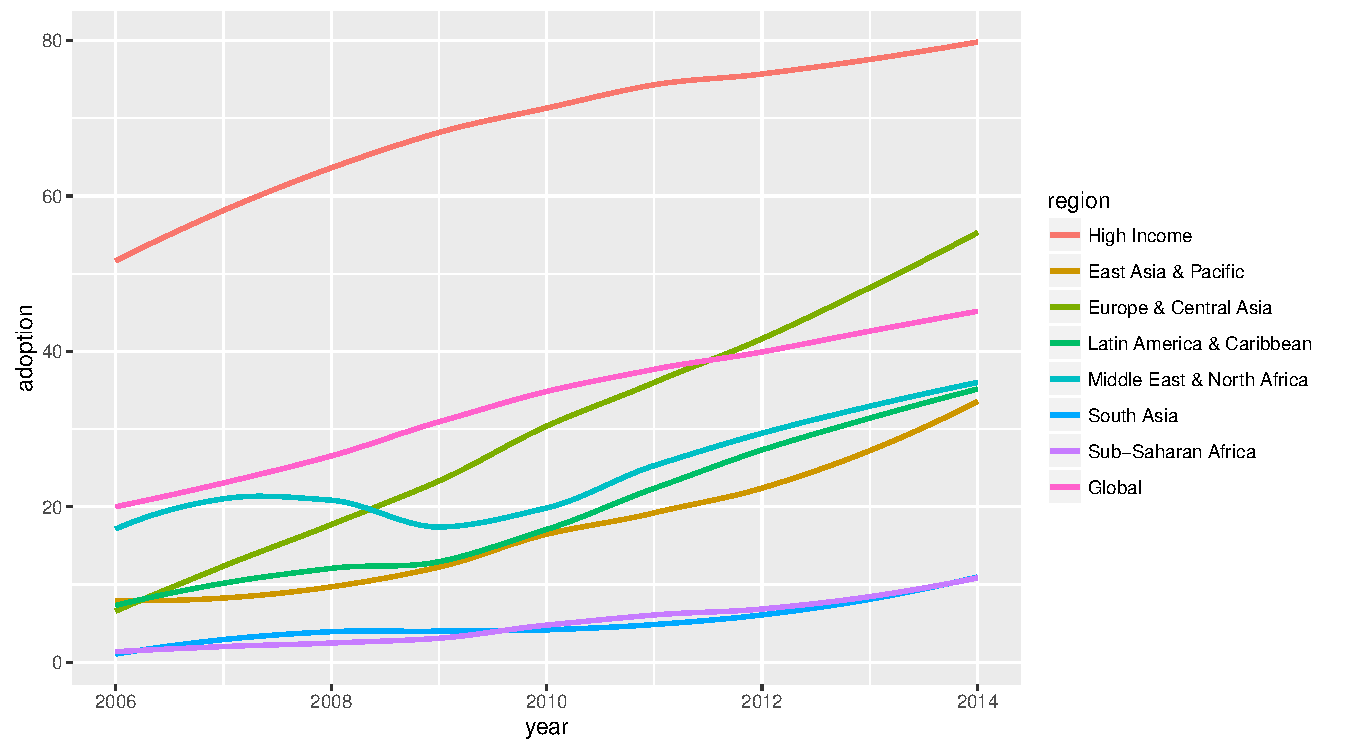
\includegraphics[width=\maxwidth]{../misc/latex-mobile_growth-1} 

\end{knitrout}
\end{figure}

A crucial factor in Internet adoption by native speakers of a language
is the interplay with content creators using that language. This dynamic
is know as a two-sided market, which is characterised as having two
different sides, which exhibit positive cross-side network effects
\citep{parker2000information,parker2000internetwork,parker2005two}.

\subsection{Two-Sided Markets}

In the case of Internet adoption in a certain language, these sides
are on the one hand the content creators, such as news websites and
on the other hand the content consumers, or Internet users. Ideally,
adoption should follow a virtuous circle, whereby the content offering
encourages more users to come online, which in turn incentivises more
content creation and so forth \citep{rochet2003platform,rochet2006two}.
Unfortunately this virtuous circle sometimes fails to properly start
for certain languages, this is especially important as it typically
concerns communities who's linguistic characterisation can already
hamper economic growth \citep{arcand2013language}. Herein also lies
the difficulty with finding empirical evidence supporting these dynamics,
since the process of adoption by users and content creators is inherently
endogenous. With this paper I seek to empirically address the question
if increased accessibility of content does indeed lead to an increase
in Internet adoption.

By considering that these markets are shaped by the protocols they
agree upon and by also viewing language as such a protocol, it emerges
that the two-sided market for Internet exists separately for each
language. We can model the differences in protocols (and language)
as transaction costs, if the linguistic barrier is significant enough,
the transaction is not conducted and agents leave the market.

A two-sided market can be defined as an economic platform with two
distinct sets of agents (in this case Internet users and content creators),
that provide each other with network effects, meaning that they provide
the other side with greater value for entering the market. 

The model of a two-sided market is a specific case of a market with
simple network effects, such as the market for telephones. In the
market for telephones, all users act as both creators and consumers
of content, by speaking and listening respectively. The more other
people have telephones, the greater the benefit derived from owning
one is, since it can connect to more people (simple network effects).

The two-sided market is a specific case, since it restricts a set
of agents to one role (e.g. transmitting) and the other agents to
a complementary role (e.g. receiving). The network effects here manifest
as a sort of seesaw, more transmitters means greater utility is derived
from being a receiver, and more receivers in turn means that greater
utility is derived from being a transmitter, etcetera. These are called
cross-side network effects and a market that exhibits them is called
a Two-Sided Market (2SM). 

\subsubsection*{Protocol Stack / Convention Ensemble}

Although often discussed as such, these markets and platforms do not
existing in isolation, but in fact build upon each other in a value
chain (much like other markets).

The Internet itself is a set of agents (computers) that are connected
to each other via a protocol called the Internet Protocol (IP). Viewed
jointly, this can be seen as a platform with simple network effects,
since additional computers in the network communicate bidirectionally.
Therefore, more computers increase the utility of owning a computer,
as it can communicate with more other computers and their users. In
this market, there is no single intermediary, since users can connect
through any ISP and will still be able to connect to any other computer
on the Internet.

\begin{table}[H]
\caption{Protocol Stack}

\centering{}%
\begin{tabular}{|c|c|}
\hline 
Social Media (simple network effects, proprietary) &
Spam (one-way network effects)\tabularnewline
\hline 
Websites (cross-side network effects) &
Email (simple network effects)\tabularnewline
\hline 
\multicolumn{2}{|c|}{TCP/IP (simple network effects)}\tabularnewline
\hline 
\end{tabular}
\end{table}

This platform is built upon by using additional protocols so that
eventually communication is conducted using a combination of protocols
called the protocol stack (in economic terms we might call this a
\textquotedbl convention ensemble\textquotedbl ). For instance,
emails are sent through protocols such as the Simple Mail Transfer
Protocol (SMTP), which builds upon the Internet Protocol. Of course,
proprietary variants of such additional platforms with simple network
effects also exists. For instance Twitter or WhatsApp behave similar
to email in many ways, but in both cases, there is only one single
intermediary that users can use to connect to the network.

These additional protocols can change the nature of the network effects,
e.g. from simple network effects to the cross-side network effects
of a two-sided market. For instance, the WWW (websites) uses the HTTP
protocol to transmit files with HTML content. In simplified view,
the HTTP protocol is designed to transmit websites from servers to
users. In this case, we thus distinguish between agents that send
content (servers/websites) and agents that receive content (users/browsers),
the two sides benefit from cross-side network effects, since more
users means a greater audience to websites and more websites means
more content to consume for users.

However, these additional protocols need not change the nature of
the market. For instance, agents that use email for communication
will both send and receive emails, making it a platform with simple
network effects, just like the Internet itself at the IP level. Particularly,
since users can chose from many email providers and still communicate
with all other users. 

\subsubsection*{General View of Protocols}

We can now use this approach of analysing the nature of the network
effects at every additional level of protocols to examine the role
of language. We return to the example of the WWW, which is a two-sided
market based on the fact that the HTTP basically works to transmit
websites from servers to users. 

These technical protocols enable the communication between the various
computers connected to the Internet in various ways. However, essentially
these computers merely fulfil a role in enabling human communication.
As such other protocols of that human-to-human communication also
play a role, chief among those is the language of writing (or speaking).

By moving beyond the technical-only interpretation of protocols, and
including language, we see that the additional protocols again lead
to the creation of distinct platforms. It is thus the case that the
two-sided market of the WWW is actually composed of many two-sided
markets in different languages (or non-linguistic communication). 

\subsubsection*{Transaction Costs}

We can interpret these differences in protocol as a form of transaction
costs \citep{coase1937nature}. Transaction costs have been broadly
defined by Steven N. S. Cheung as: \textquotedbl any costs that are
not conceivable in a \textquotedbl Robinson Crusoe economy\textquotedbl .
We can interpret this as costs that stem from the presence of institutions
or conventions.

For instance, consider the way in which people answer a fixed-line
telephone. Since the phone is shared by the household, the person
calling does not know who will answer the phone, it is therefore customary
to state your name when you answer the telephone. With the rise of
mobile phones, people who did not have mobile phones or used them
less expected people to answer them the same way you answer a fixed-line
phone, by stating your name, but people who did use mobile phones
quickly realised that it could only logically be expected that they
would be the one answering the phone, eliminating the need to state
your name and use just \textquotedbl hello\textquotedbl{} instead.
This was a partial breakdown of protocol. We can interpret this as
transaction costs, if the person calling was sufficiently confused
by not being told who they are speaking to, he/she might hang up the
phone. Alternatively, they might feel offended and irritant, making
the conversation less effective or possibly cutting it short.

Similar things apply to technical protocols. For instance, consider
the introduction of something like a new HTML tag, this tag will be
interpretable by new browsers that support these tags, but not by
older browsers, causing the older browsers to misrender part of the
page. Depending on the gravity, this might make the page harder to
view, or simply impossible. Similarly, old tags are sometimes deprecated
(e.g. IE6 specific tags), which means that they can no longer be interpreted
by newer browsers (e.g. IE10), giving similar results. The transactions
costs might thus be sufficient to stop communication, or simply hinder
it. If the hindering continues, it might be that the users consumers
a smaller amount of content.

Language can also be interpreted as a protocol or convention for communication
and we can therefore also interpret linguistic differences as a transaction
cost.

Intuitively we might think of language as a discrete variable, perhaps
making transactions costs a poor way to approximate this. However,
there are many cases in which linguistic differences are a definite
barrier, but not necessarily a breaking point. For instance, a Portuguese
speaker might be able to read a Spanish website if Portuguese is not
available, but they would always have less effort in reading Portuguese
(and thereby consume more). This transaction cost would increase if
we consider for instance an Italian speaker reading Spanish. Moving
to a French speaker reading Spanish, which is really quite distinct,
but nevertheless some similarity in terms of vocabulary. Moving to
a different language family, such as German, the differences probably
become insurmountable. For a Japanese speaker not a single word would
be meaningful. This is especially the case, as the Japanese speaker
in question would not understand the latin script. 

If we assume that the Internet's value only stems from communicating
with other people, then we might define a utility function like this: 

\begin{equation}
u_{i}()=-p+\sum_{j=1}^{n}d_{ij}l_{ij}v_{ij}c_{j}
\end{equation}

Whereby p represents the cost of connecting to the Internet and the
the other term is the value of all possible connections to all individuals.
Here, $v_{ij}$ represents the value of the connection between individual
$i$ and $j$, to individual $i$. This is multiplied with the $l_{ij}$
term, which is the likelihood that individuals $i$ and$j$ will establish
a connection given that they both have Internet connectivity. This
is again multiplied by the $d_{ij}$ term, which represents the difficulty
of communication between individuals $i$ and $j$, Finally, this
is multiplied with the decision of $j$ to connect to the Internet
or not $c_{j}$ ,where $c_{j}\in{0,1}$. Of course this decision in
turn depends on the utility of connecting to $j$, where $w_{j}\in{0,1}$.
The term $w_{j}$ represent whether it is worth it or not to connect:

\begin{equation}
c_{j}()=w_{j}(-p+\sum_{k=1}^{n}d_{jk}l_{jk}v_{jk}c_{k})
\end{equation}

Which means if:

\begin{equation}
p<\sum_{k=1}^{n}d_{jk}l_{jk}v_{jk}c_{k}
\end{equation}

then $w_{j}=1$, otherwise $w_{j}=0$.

The move from simple network effects to the cross-side network effects
is made when the ease of communication variable $d_{ij}$ stays high,
but $d_{ji}$ becomes very low (e.g. HTTP). This means that is would
be relatively easy for a certain type of agent (server) to communicate
something to another type of agent (Internet user), but that reverse
communication is less easy. In the context of language we could consider
a Spanish speaker who could communicate something to a Portuguese
speaker, if the Portuguese speaker has some passive understanding
of Spanish. But that this communication cannot be reversed, since
the Portuguese speaker does not have an active understanding or Spanish
and the Spanish speaker does not have a passive understanding of Portuguese.
Note that a market can also become two-sided if the information being
communicated is different (e.g. buy vs. selling a product).

When communication breaks down in both directions, then markets start
to exist parallely. For instance, in the above example, if the Portuguese
speaker loses his passive understanding of Spanish, then they cease
to operate in a common market, rather they each operate in a separate
- parallel - market, in this case a Portuguese-language market for
communication and a Spanish-language market for communication.

The nature of these parallel markets is again determined by the protocols
that they use. For instance, the market of Portuguese-language websites,
is a two-sided market, based on the fact that the underlying HTTP
protocol functions so.

These transaction costs could possibly explain why the automatic optimal
allocation of resources (according to the Coase theorem) does not
allocate any to groups with certain languages (even if the resource
- i.e. space on the Internet - is virtually unlimited).

\section{Data}

\label{sec:data}The National Income Dynamics Study (NIDS) collects
data on a representative set of around ten thousand South African
households across several time periods. The first wave was gathered
in 2008, the second wave in 2010, and the third wave was gathered
in 2012 \citep{saldru2008nids,saldru2012nids,saldru2013nids}.

In addition to this, in may 2016 a fourth wave of data has also been
partially published, which I used to relate the expanded demographic
of Setswana speaking Internet users to improvements in employment
levels.

The dataset contains an extensive household questionnaire, which contains
detailed information on income and expenditure. In particular, it
breaks household expenditure down into many forms of food and non-food
expenditure, one of which is household expenditure on Internet access
in the last 30 days. In addition to this, the household income is
calculated and imputed with other income such as home ownership. The
individual (adult) questionnaires also contain information on linguistic
skills in both English and in the interviewees native language, as
well as a series of variables relating to communication technology
ownership and utilisation, in particular computer ownership. In \tabref{dep_vars}
an overview of the dependent variables, broken down by wave and native
language is presented.



\begin{table}[H]

\caption{Dependent Variable Descriptive Statistics}

\begin{centering}
\begin{tabular}{|l|r|r|r|}
\hline 
 &
Wave &
Setswana &
Other\tabularnewline
\hline 
\hline 
Computer Ownership &
1 &
0.0351 &
0.0567\tabularnewline
\hline 
 &
2 &
0.0359 &
0.0417\tabularnewline
\hline 
 &
3 &
0.0711 &
0.0632\tabularnewline
\hline 
Household Internet Expenditure &
1 &
0.0068 &
0.0162\tabularnewline
\hline 
 &
2 &
0.0037 &
0.0224\tabularnewline
\hline 
 &
3 &
0.0106 &
0.0140\tabularnewline
\hline 
\end{tabular}
\par\end{centering}
\end{table}

I use both household expenditure on Internet access and computer ownership
as dependent variables. Household expenditure includes a variety of
way in which this expense can be made, including paying for a fixed-line
subscription, a mobile Internet subscription, as well using Internet
in an Internet cafe. More than 99\% of South Africa is covered by
mobile Internet networks, this figure did not change during the time
periods used in this study \citep{international2015world}. Computer
ownership is recorded in the individual adult questionnaire, which
provides me with more observations, unlike expenditure in the last
30 days, this shows a more long-term investment.

In addition to the variables of interest, I include a number of relevant
covariates, such as household income and education levels. Furthermore,
I include information on English and native language reading and writing
skills. Around 45\% of the individuals report being able to read and
write English fluently, whereas around 55\% report being able to do
so in their native language.

In \ref{fig:langsex} we can see the number of native speakers for
each language in the dataset, coloured by gender. The dataset contains
a total of 51,612 observations (adult individuals), of which 2,806
are female native Setswana speakers and 2,140 are male native Setswana
speakers.

\begin{figure}[H]
\caption{Native Language and Gender}

\label{fig:langsex}

\begin{knitrout}
\definecolor{shadecolor}{rgb}{0.969, 0.969, 0.969}\color{fgcolor}
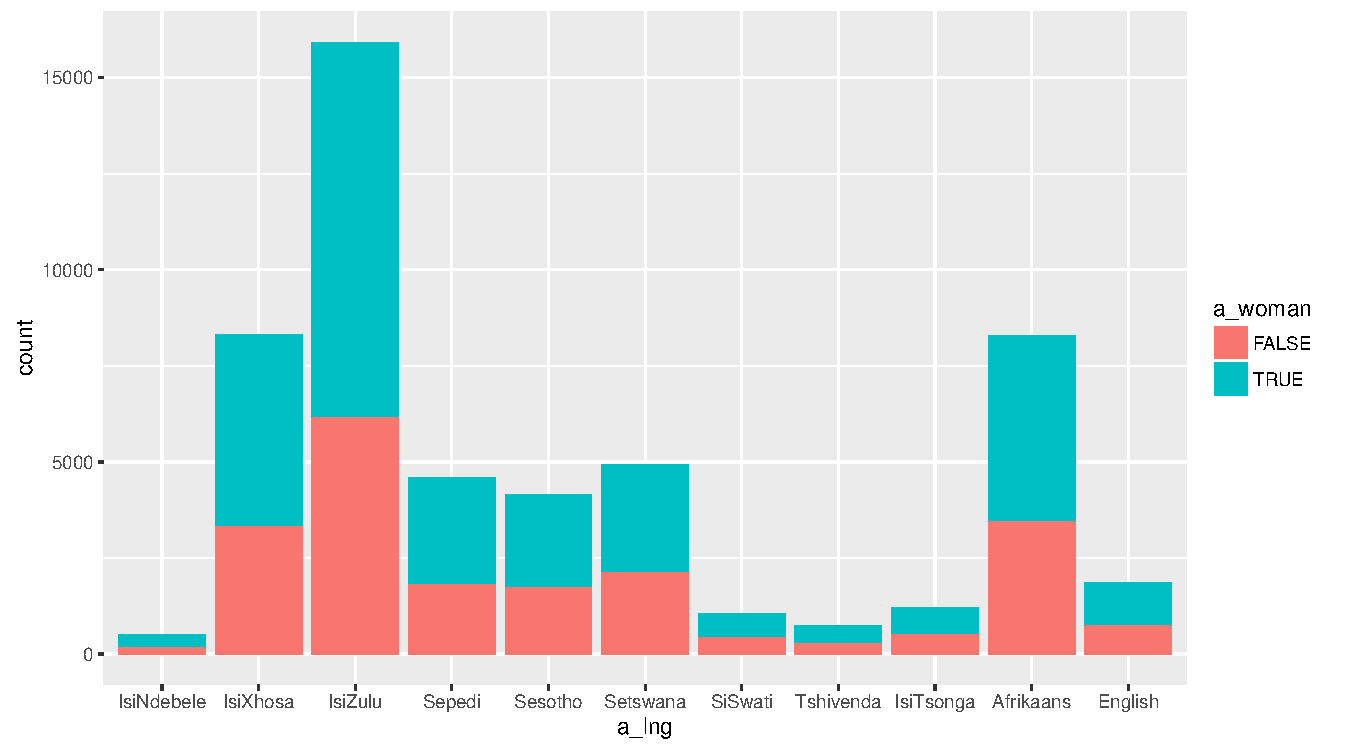
\includegraphics[width=\maxwidth]{../misc/latex-lang_woman-1} 

\end{knitrout}
\end{figure}


\section{Empirical Methodology}

\label{sec:methods}With this paper I aim to answer the question whether
increased content or accessibility of content leads to an increase
in demand. This section begins with a discussion of the identification
strategy employed, followed by a explanation of the estimator used
to operationalise this.

\subsection{Identification Strategy}

\label{subsec:identification}This paper exploits the introduction
of the Setswana interface language to Google Search in South Africa
as a spillover of the development of that interface for the Botswanan
Google Search website. By comparing the number of native Setswana
speakers in South Africa being Internet users, with the number of
South Africans with a different native language around the same time,
I isolate the effect of this introduction.

The Setswana language interface was first developed for the Botswanan
Google Search website (\code{google.co.bw}). As such, the introduction
of Setswana to the South African Google Search (\code{google.co.za})
was a spillover effect of that development. This allows me to rule
out any possible endogeneity issues that might otherwise arise in
contexts such as these. For instance, the Afrikaans language is almost
solely spoken in South Africa. When we observe that the introduction
of the Afrikaans Google Search interface occurs around the same time
as a growth in the number of native Afrikaans Internet users, it will
be hard to isolate the effect from the introduction from its cause
(since an increase in native Afrikaans Internet users would be a good
reason to introduce it as an interface language).

Substantial numbers of Setswana speakers exist in Botswana, South
Africa, Zimbabwe, and to some extend Namibia. However, the language
is most important in Botswana, where it is spoken by approximately
80\% of all people, and where it is the only official language other
than English. As such, it is also the place where most linguistic
work on the Setswana language takes place. The Setswana Google Search
interface was also developed at the University of Botswana by prof.
Otlogetswe.

It is worth noting that it is very common to not personally own a
computer, therefore `paying for Internet access' also includes a lot
of people who use the Internet in other locations such as Internet
cafe's.

In addition to using the propensity to spend on Internet (in the last
thirty days), I also use the propensity to own a computer as a dependent
variable. 

\subsection{Regression Specification}

\label{subsec:estimation}As mentioned in the above section, I compare
the change in the level of Internet users among native Setswana speakers
in South Africa, with that of native speakers of other language in
South Africa around the introduction of the Setswana interface to
the South-African Google Search, after the second wave of the NIDS.
For this I use a Difference-in-Differences estimator \citep{abadie2005semiparametric,imbens2009econometrics}
using a native-Setswana speaker dummy variable (\code{setswana}),
interacted with an event dummy variable (\code{event}). The former
is \code{TRUE} when the native language of the individual (\code{a\_lng})
is \code{Setswana} and \code{FALSE} otherwise. The latter is \code{FALSE}
for data collected prior to the introduction of the Setswana interface
language (late 2010, here wave 1 and 2) and \code{TRUE} after this
introduction (here wave 3). The model than takes the form as described
in \eqref{m1}.

\begin{equation}
y_{it}=\alpha_{i}+\lambda_{t}+\delta D{}_{it}+\beta X_{it}+\epsilon_{it}\label{eq:m1}
\end{equation}

Where $\alpha_{i}$ represents the individual fixed effects, $\lambda_{t}$
represent the time fixed effects, and $X_{it}$ are the time varying
covariates. The $\epsilon_{it}$ is the error term. Finally the term
of interest is $D_{it}$ which represents the treatment effect.

The \code{h\_nfnet} variable is recorded at a household level, as
such a standard error correction needs to be applied \citep{white1980heteroskedasticity},
the model with standard error corrections is reported in the appendix.

Lastly, the dependent variables are both logical or binary variables,
as such, normally a model such as logit should be used. However, since
I am using Difference-in-Differences, this model would be undefined
\citep{wooldridge2010econometric}, I therefore use a standard linear
model. 

\section{Results}

\label{sec:results}In the base model, I use an interaction of the
\code{event} dummy and \code{setswana} dummy in order to isolate
the effect on the explanandum, a dummy variable describing household
expenditure on Internet in the last thirty days or not (\code{Internet\_expenditure},
household non-food Internet). The results of this estimation are presented
in \tabref{esti-full}.

I find that the interaction term of the event dummy (\code{event})
and the native Setswana speaker dummy (\code{setswana}) is positive
and highly significant, with a p-value around \code{0.0018}. Both
the individual dummy variables (\code{event} and \code{setswana})
yield significant negative parameter estimates.

In addition to this, the covariates included in the estimation are
also highly significant. The highest education level of the individual
(\code{best\_edu}) and the household income (\code{hhincome}) are
both positive and significant. The parameter estimate of \code{woman}
here is negative but not at all significant, this is unsurprising
as I use Internet expenditure at a household level. Most women live
in a household which includes men and visa versa, suggesting that
this effect cannot be isolated in this estimation. I further investigate
this issue in a separate estimation discussed below. The variables
describing linguistic skills in reading and writing in both English
and the native language do yield many significant results, though
lower levels of English writing skill seems to be correlated with
a lower propensity to use the Internet (\code{a\_edlitwrten} for
levels \code{2} and \code{3}, but not the very lowest: \code{4}).

In an alternative formulation, I include the native language variable
as a categorical variable (\code{language}), interacted with the
\code{event} dummy. In this estimation I only find significantly
positive results for \code{Setswana} and \code{Venda} (as small
language from the region bordering Zimbabwe), and a significantly
negative effect for the language \code{Afrikaans}.

When using the propensity of adults (\code{own\_computer}) to own
a computer is used as an explanandum, I find similar results. This
is of particular relevance, as the explanandum here (\code{own\_computer})
differs from the base model's explanandum in two ways. Firstly, it
does not include expenditure on Internet in ways such as Internet
cafes, but focusses on actual ownership, signalling a more long-term
investment and interest. Secondly, the \code{Internet\_expenditure}
variable is at a household level, whereas the \code{own\_computer}
variable is at the level of an individual adult. The results from
this estimation are included in \tabref{esti-full}. This form of
the estimation yields similar results to those estimated in the base
model. Firstly I find that the variable of interest, the interaction
term between the event and the language dummy (\code{event {*} setswana})
is positive at 0.024 and highly significant, with a p-value smaller
than \code{0.001}. This means that the event increased the propensity
to own a computer by 2.4\%. The individual dummy variables (\code{event}
and \code{setswana}) again are significant and negative with the
former's p-value smaller than \code{0.01} and the latter's smaller
than \code{0.001}. In terms of the linguistic skill, I find that
the lower levels of English reading as well as English writing are
correlated with lower propensities of computer ownership. Similar
to Internet expenditure model, household income (\code{hhincome})
and highest level of education (\code{best\_edu}) are both positive
and highly significant (p-value: \code{\textasciitilde 0}). However,
unlike in the household Internet expenditure model, the gender of
the individual here is highly significant, specifically, parameter
estimate of \code{woman} is negative and highly significant (p-value:
\code{\textasciitilde 0}). As mentioned above, this variable is difficult
to interpret when using a household-level variable as an explanandum,
however, here, the computer ownership variable is at an individual
level, which makes the coefficient more easily interpretable.

\begin{table}

\caption{Internet Access and Computer Ownership}

\begin{centering}
\label{tab:esti-full}
\par\end{centering}
\centering{}%
\begin{tabular}{|l|r|c|c|c|}
\hline 
 &
Internet &
(P > |t|) &
Computer &
(P > |t|)\tabularnewline
\hline 
\hline 
event {*} setswana &
0.012 &
0.003 &
0.024 &
0.005\tabularnewline
\hline 
event &
-0.011 &
0.001 &
-0.006 &
0.001\tabularnewline
\hline 
setswana &
-0.013 &
0.002 &
-0.0155 &
0.004\tabularnewline
\hline 
income (10,000 ZAR) &
0.270 &
0.000 &
0.540 &
0.000\tabularnewline
\hline 
woman &
-0.001 &
0.001 &
-0.027 &
0.014\tabularnewline
\hline 
education &
0.001 &
0.000 &
0.006 &
0.000\tabularnewline
\hline 
Observations &
87634 &
 &
87634 &
\tabularnewline
\hline 
\end{tabular}
\end{table}

The below figure presents a graphical illustration of the above mentioned
result. As we can see, initially, the propensity to own a computer
for setswana speakers (blue line) was similar to the average of speakers
of other languages (red line), however after the introduction of the
Setswana language search interface, between waves 2 and 3, we observe
a sharp increase in this propensity for setswana speakers in wave
3, whereas average of other languages remains relatively unchanged.

\begin{figure}[H]
\caption{Computer Ownership Setswana}

\begin{knitrout}
\definecolor{shadecolor}{rgb}{0.969, 0.969, 0.969}\color{fgcolor}
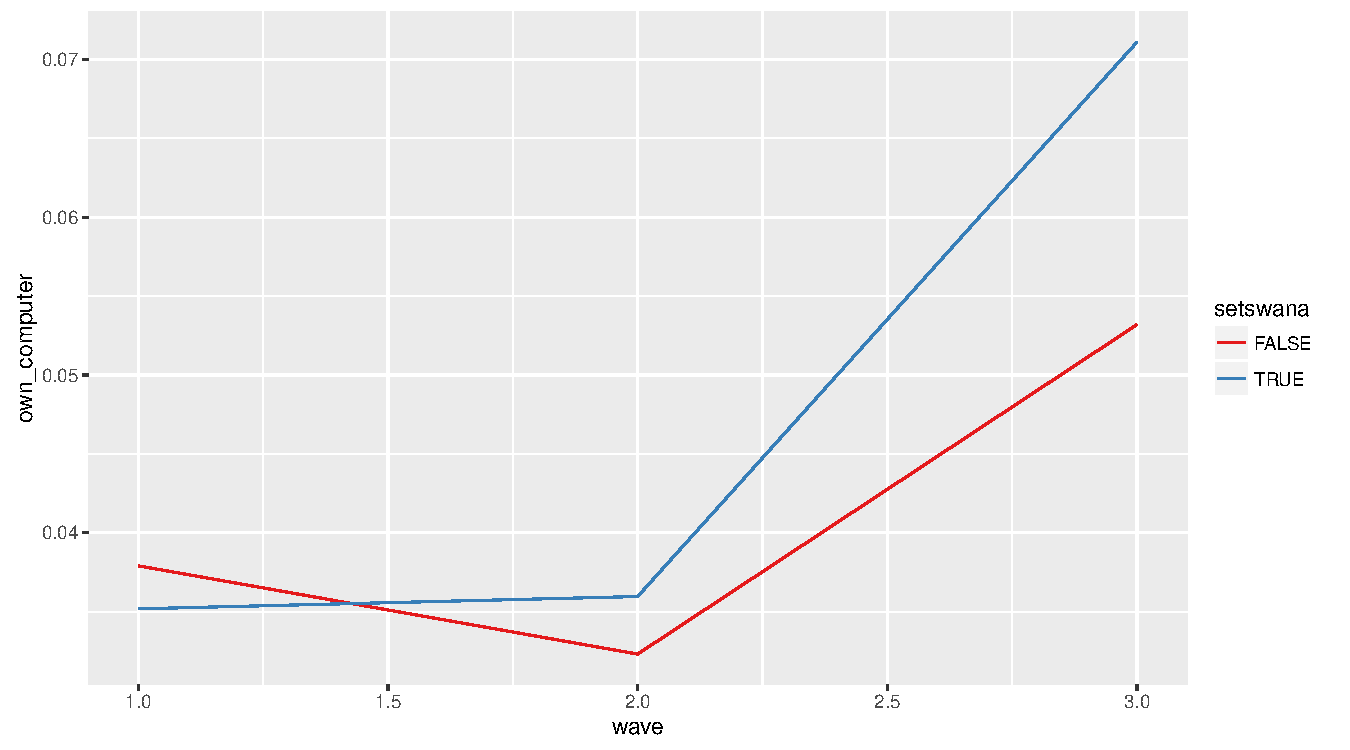
\includegraphics[width=\maxwidth]{../misc/latex-gg2_5-1} 

\end{knitrout}
\end{figure}

I also plot this variable separately for each gender.

\begin{figure}[H]
\caption{Computer Ownership Setswana by Gender}

\begin{knitrout}
\definecolor{shadecolor}{rgb}{0.969, 0.969, 0.969}\color{fgcolor}\begin{kframe}


{\ttfamily\noindent\bfseries\color{errorcolor}{\#\# Error in grouped\_df\_impl(data, unname(vars), drop): Column `woman` is unknown}}\end{kframe}
\end{knitrout}
\end{figure}

I estimate the effect of the introduction specifically on setswana
speaking women, by interacting the woman binary variable with the
above used interaction term between the event dummy and the Setswana
language dummy. The effect is strongly negative with a value of -0.025.
The interaction term between the event and the language dummy (i.e.
for men, since woman==FALSE) is strongly positive at 0.038. Combining
these two effects gives us the estimated effect on the event on woman,
0.038 - 0.025 = 0.013, which is roughly a third of men (0.038). The
interaction term between woman and setswana is slightly positive at
0.009, which means that Setswana speaking women are on average slightly
more likely to own a computer than woman in general are.

\begin{table}[H]

\caption{Women and Computer Ownership}

\begin{centering}
\begin{tabular}{|l|r|r|}
\hline 
 &
Computer &
(P > |t|)\tabularnewline
\hline 
\hline 
woman {*} event {*} setswana &
-0.025 &
0.011\tabularnewline
\hline 
event {*} setswana &
0.038 &
0.008\tabularnewline
\hline 
event &
-0.002 &
0.006\tabularnewline
\hline 
setswana &
-0.021 &
0.007\tabularnewline
\hline 
income (10,000 ZAR) &
0.054 &
0.000\tabularnewline
\hline 
woman &
-0.021 &
0.003\tabularnewline
\hline 
education &
0.006 &
0.000\tabularnewline
\hline 
woman {*} setswana &
0.009 &
0.009\tabularnewline
\hline 
woman {*} event &
-0.007 &
0.003\tabularnewline
\hline 
Observations &
87634 &
\tabularnewline
\hline 
\end{tabular}
\par\end{centering}
\end{table}

\ref{fig:GoogleTrendsZA}, illustrates how usage of the Setswana word
`thuso', meaning `help' in search queries, was zero prior to the introduction
of the Setswana search interface and became widespread thereafter.
Therefore, in addition to the increased Internet usage by Setswana
speakers, we can also observe an increased usage of the Setswana language
itself. This can lead to greater amounts of Setswana language content
being found and engaged with, which in turn incentivised content creators
to provide more Setswana language content. This could help break the
vicious circle of low levels of content and few users.

\begin{figure}[H]
\caption{Usage of Setswana Words on Google.co.za}

\begin{centering}
\label{fig:GoogleTrendsZA}
\par\end{centering}
\begin{centering}
\par\end{centering}
\centering{}\includegraphics[scale=0.48]{0_home_bquast_Making-Next-Billion-Demand-Access_misc_thuso.pdf} 
\end{figure}

As mentioned in \secref{data} I use the partially released 4th wave
of the dataset, which covers the year 2014 in order to relate the
increased Internet usage with employment levels. I do this by subsetting
data to include one the one hand, only the individuals that owned
a computer in after the event in wave 3 and on the other hand the
individuals in households that reported spending on internet access.
The idea is that the owners/users in wave 3 are an expanded demographic
for Setswana speakers but remain relatively unchanged. With this,
we can see the evolution of the employment level for this expanded
demographic.

In the below figure, I plot the employment status of individuals that
own a computer in the first wave after the introduction of the Setswana-language
interface (wave 3). The figure shows that there is a sharp uptick
in thdisenfranchisemente proportion of employed individuals among
Setswana speakers. 

\begin{figure}[H]
\caption{Employment for Individuals who Own a Computer in Wave 3}

\begin{knitrout}
\definecolor{shadecolor}{rgb}{0.969, 0.969, 0.969}\color{fgcolor}
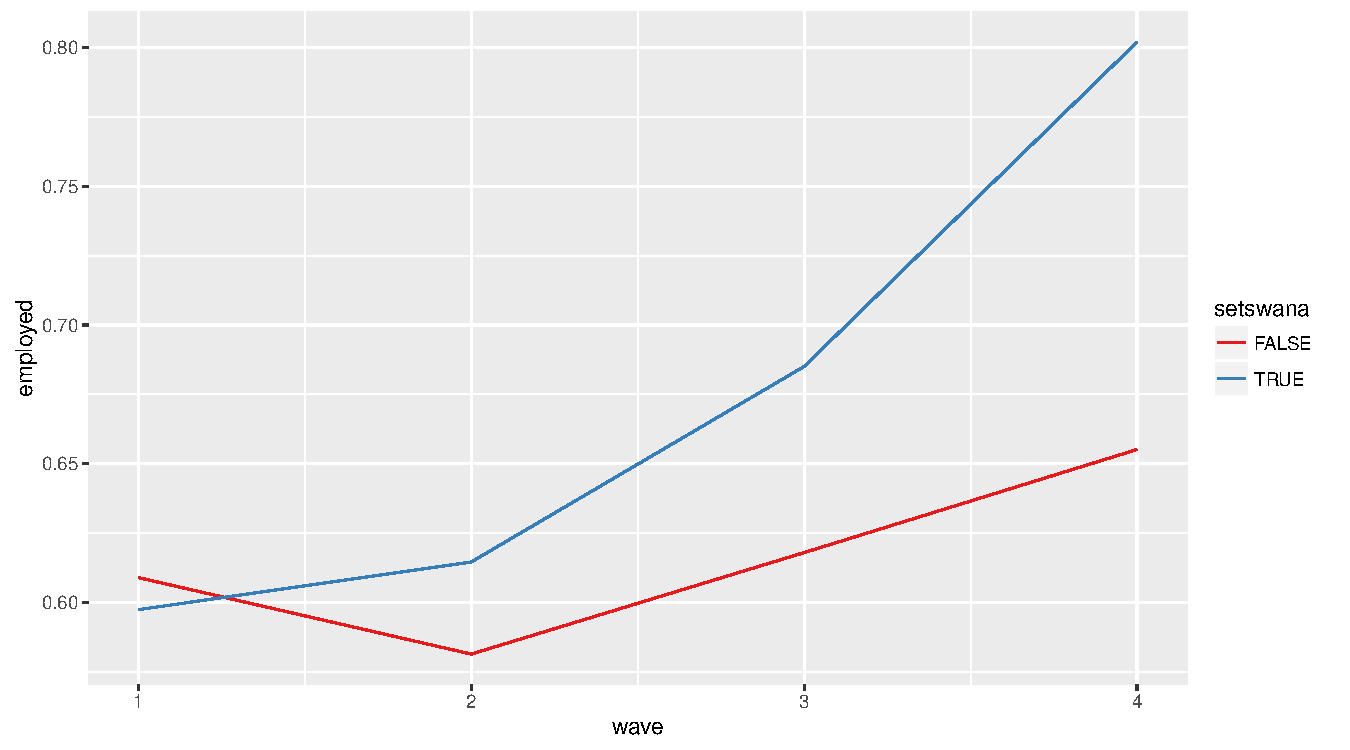
\includegraphics[width=\maxwidth]{../misc/latex-employment_own_computer-1} 

\end{knitrout}
\end{figure}

Similarly, the individuals that lived in a household that spent on
Internet access in the last 30 days also saw a strong increase in
the proportion of employed individuals, overtaking the proportion
for the rest of the population.

\begin{figure}[H]
\caption{Employment for Individuals with Internet Expenditure in Wave 3}

\begin{knitrout}
\definecolor{shadecolor}{rgb}{0.969, 0.969, 0.969}\color{fgcolor}
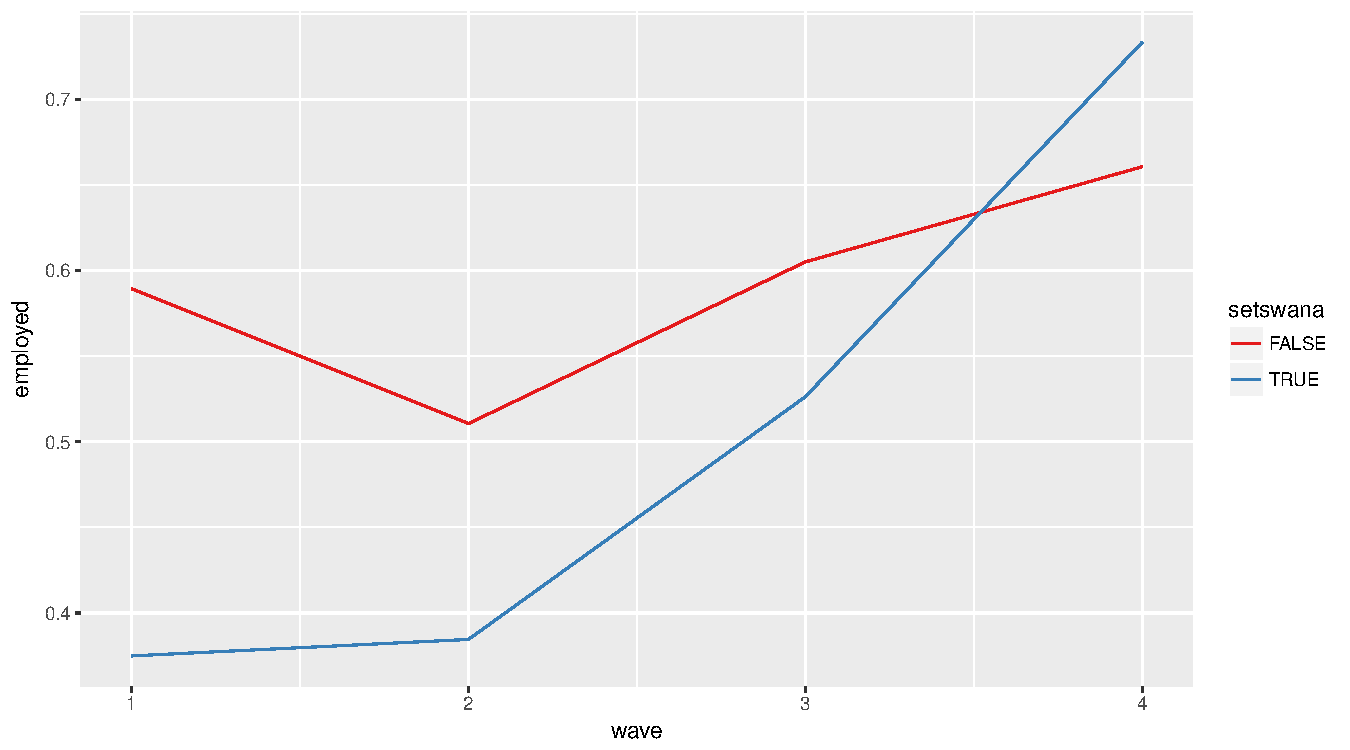
\includegraphics[width=\maxwidth]{../misc/latex-employment_int_exp-1} 

\end{knitrout}
\end{figure}

Finally we can plot the above graphs for men and women separately.

\begin{figure}[H]
\caption{Employment for those owning a Computer in Wave 3 by gender}

\begin{knitrout}
\definecolor{shadecolor}{rgb}{0.969, 0.969, 0.969}\color{fgcolor}\begin{kframe}


{\ttfamily\noindent\bfseries\color{errorcolor}{\#\# Error in grouped\_df\_impl(data, unname(vars), drop): Column `woman` is unknown}}\end{kframe}
\end{knitrout}
\end{figure}

\begin{figure}[H]
\caption{Employment for those with Internet Expenditure in Wave 3 by gender}

\begin{knitrout}
\definecolor{shadecolor}{rgb}{0.969, 0.969, 0.969}\color{fgcolor}\begin{kframe}


{\ttfamily\noindent\bfseries\color{errorcolor}{\#\# Error in grouped\_df\_impl(data, unname(vars), drop): Column `woman` is unknown}}\end{kframe}
\end{knitrout}
\end{figure}


\section{Conclusions and Limitations}

\label{sec:conclusions}In conclusion, despite recent advances in
the reach, speed, and affordability of Internet connectivity in sub-Saharan
Africa, actual uptake has been stagnant. Internet adoption is a two-sided
market, as a result, one aspect of this is that users benefit from
cross-side network effects from content. Unfortunately, in certain
languages, a sufficient amount of content is not always created, as
a result, Internet adoption among native speakers of these languages
can lag behind.

This paper demonstrates that this failure can in part be attributed
to the dynamics of a two-sided market, whereby the vicious circle
of few users and little content perpetuates a situation of low levels
of adoption. Due to the endogenous nature of two-sided markets, there
are few methods of isolating a causal effect.

I exploit the introduction of the Setswana-language interface on \code{google.co.za},
as a spillover of the development of this interface for \code{google.co.bw},
I find that it leads to a substantial increase in Internet usage and
computer ownership among native Setswana speakers.

Furthermore, when comparing the Setswana speakers that own a computer
or spend on Internet access after the event, with non Setswana speakers,
we see a marked increase in the proportion of employed individuals
over that among the rest of the population. This increase is even
stronger in wave 4 of the data, suggesting that it takes some time
for the effect to fully materialise and that it is persistent.

This increase of Internet usage among the Setswana speaking population
as a result of the newly introduced interface language on \code{google.co.za},
suggests that there is a serious lack in the availability of local
content in many indigenous African languages, which serves as an impediment
to further Internet adoption. 

 This suggests that the effect is unlikely to be ephemeral in nature,
since computer ownership constitutes a more long-term investment in
Internet access.

As I discussed in the results section, the increase in computer ownership
for Setswana speakers between wave 2 and wave 3, was 115\%, compared
to 70\% for the rest of the population, or a 50\% greater increase.
The effect on Internet expenditure in the household, which includes
expenditure in Internet cafes etc. is even greater. The proportion
of Setswana households that spent on Internet in the last 30 days
increased by 217\%, whereas for the rest of the population it fell
be 22\%.

\newpage{}

\printbibliography


\appendix

\section{Clustering}

\begin{table}[H]
\caption{Clustering}

\begin{knitrout}
\definecolor{shadecolor}{rgb}{0.969, 0.969, 0.969}\color{fgcolor}\begin{kframe}
\begin{alltt}
\hlkwd{library}\hlstd{(plm)}    \hlcom{# panel linear model estimation}
\hlkwd{library}\hlstd{(lmtest)} \hlcom{# Standard Error corrections}
\hlkwd{library}\hlstd{(broom)}  \hlcom{# output formatting using tidy()}

\hlcom{# specify panel model}
\hlstd{plm4_3} \hlkwb{<-} \hlkwd{formula}\hlstd{(}\hlkwd{as.numeric}\hlstd{(h_nfnet)}  \hlopt{~} \hlstd{interface_intro}\hlopt{*}\hlstd{setswana}  \hlopt{+}
                                         \hlkwd{factor}\hlstd{(a_edlitrden)}  \hlopt{+}
                                         \hlkwd{factor}\hlstd{(a_edlitwrten)} \hlopt{+}
                                         \hlkwd{factor}\hlstd{(a_edlitrdhm)}  \hlopt{+}
                                         \hlkwd{factor}\hlstd{(a_edlitwrthm)} \hlopt{+}
                                         \hlstd{a_woman}              \hlopt{+}
                                         \hlstd{hhincome}             \hlopt{+}
                                         \hlstd{best_edu              )}
\hlcom{# estimate}
\hlstd{plm4_3e} \hlkwb{<-} \hlkwd{plm}\hlstd{(plm4_3,} \hlkwc{data}\hlstd{=pNIDS,} \hlkwc{model}\hlstd{=}\hlstr{'within'}\hlstd{)}
\end{alltt}


{\ttfamily\noindent\bfseries\color{errorcolor}{\#\# Error in `row.names<-.data.frame`(`*tmp*`, value = c("{}301012-1"{}, "{}301012-2"{}, : duplicate 'row.names' are not allowed}}\begin{alltt}
\hlcom{# correct errors}
\hlkwd{tidy}\hlstd{(} \hlkwd{coeftest}\hlstd{(plm4_3e,} \hlkwc{vcov}\hlstd{=}\hlkwd{vcovHC}\hlstd{(plm4_3e,}
                                    \hlkwc{type}\hlstd{=}\hlstr{"HC0"}\hlstd{,}
                                    \hlkwc{cluster}\hlstd{=}\hlstr{"group"}\hlstd{)) )}
\end{alltt}


{\ttfamily\noindent\bfseries\color{errorcolor}{\#\# Error in coeftest(plm4\_3e, vcov = vcovHC(plm4\_3e, type = "{}HC0"{}, cluster = "{}group"{})): object 'plm4\_3e' not found}}\end{kframe}
\end{knitrout}
\end{table}


\section{Dependent Variable Breakdown}

\begin{table}[H]
\caption{Descriptive statistics on Ownership and Expenditure}
\label{tab:dep_vars}
\centering{}
\begin{knitrout}
\definecolor{shadecolor}{rgb}{0.969, 0.969, 0.969}\color{fgcolor}


\begin{tabular}{l|r|r|r}
\hline
a\_lng & wave & a\_owncom & h\_nfnet\\
\hline
IsiNdebele & 1 & 0.0331126 & 0.0000000\\
\hline
IsiNdebele & 2 & 0.0270270 & 0.0284091\\
\hline
IsiNdebele & 3 & 0.0333333 & 0.0000000\\
\hline
IsiNdebele & 4 & 0.0532319 & NaN\\
\hline
IsiXhosa & 1 & 0.0112269 & 0.0012043\\
\hline
IsiXhosa & 2 & 0.0186335 & 0.0054517\\
\hline
IsiXhosa & 3 & 0.0345622 & 0.0019763\\
\hline
IsiXhosa & 4 & 0.0372470 & NaN\\
\hline
IsiZulu & 1 & 0.0132693 & 0.0013730\\
\hline
IsiZulu & 2 & 0.0127882 & 0.0086473\\
\hline
IsiZulu & 3 & 0.0251126 & 0.0045006\\
\hline
IsiZulu & 4 & 0.0383356 & NaN\\
\hline
Sepedi & 1 & 0.0265273 & 0.0048309\\
\hline
Sepedi & 2 & 0.0226818 & 0.0021994\\
\hline
Sepedi & 3 & 0.0718697 & 0.0050477\\
\hline
Sepedi & 4 & 0.0805596 & NaN\\
\hline
Sesotho & 1 & 0.0366044 & 0.0062598\\
\hline
Sesotho & 2 & 0.0457010 & 0.0213640\\
\hline
Sesotho & 3 & 0.0949535 & 0.0113032\\
\hline
Sesotho & 4 & 0.1025924 & NaN\\
\hline
Setswana & 1 & 0.0351724 & 0.0068681\\
\hline
Setswana & 2 & 0.0359537 & 0.0037783\\
\hline
Setswana & 3 & 0.0711086 & 0.0106264\\
\hline
Setswana & 4 & 0.0814226 & NaN\\
\hline
SiSwati & 1 & 0.0441640 & 0.0000000\\
\hline
SiSwati & 2 & 0.0612813 & 0.0091185\\
\hline
SiSwati & 3 & 0.0458221 & 0.0134771\\
\hline
SiSwati & 4 & 0.0762332 & NaN\\
\hline
Tshivenda & 1 & 0.0334928 & 0.0000000\\
\hline
Tshivenda & 2 & 0.0000000 & 0.5441176\\
\hline
Tshivenda & 3 & 0.0225080 & 0.0000000\\
\hline
Tshivenda & 4 & 0.0808625 & NaN\\
\hline
IsiTsonga & 1 & 0.0235294 & 0.0000000\\
\hline
IsiTsonga & 2 & 0.0118483 & 0.0932836\\
\hline
IsiTsonga & 3 & 0.0397196 & 0.0023529\\
\hline
IsiTsonga & 4 & 0.0776892 & NaN\\
\hline
Afrikaans & 1 & 0.1345441 & 0.0465116\\
\hline
Afrikaans & 2 & 0.0904233 & 0.0424528\\
\hline
Afrikaans & 3 & 0.1107348 & 0.0399729\\
\hline
Afrikaans & 4 & 0.1096479 & NaN\\
\hline
English & 1 & 0.2969374 & 0.1016043\\
\hline
English & 2 & 0.3234127 & 0.1070707\\
\hline
English & 3 & 0.3156934 & 0.1023766\\
\hline
English & 4 & 0.3233333 & NaN\\
\hline
\end{tabular}
\end{knitrout}
\end{table}


\section{Covariate Descriptive Statistics}

\begin{figure}[H]
\caption{Household Income}

\label{fig:hhincome}

\begin{knitrout}
\definecolor{shadecolor}{rgb}{0.969, 0.969, 0.969}\color{fgcolor}\begin{kframe}
\begin{alltt}
\hlkwd{ggplot}\hlstd{(adulthh,} \hlkwd{aes}\hlstd{(}\hlkwc{x}\hlstd{=hhincome,} \hlkwc{fill}\hlstd{=a_lng ))} \hlopt{+}
    \hlkwd{stat_bin}\hlstd{(}\hlkwc{bins}\hlstd{=}\hlnum{50}\hlstd{)}
\end{alltt}
\end{kframe}
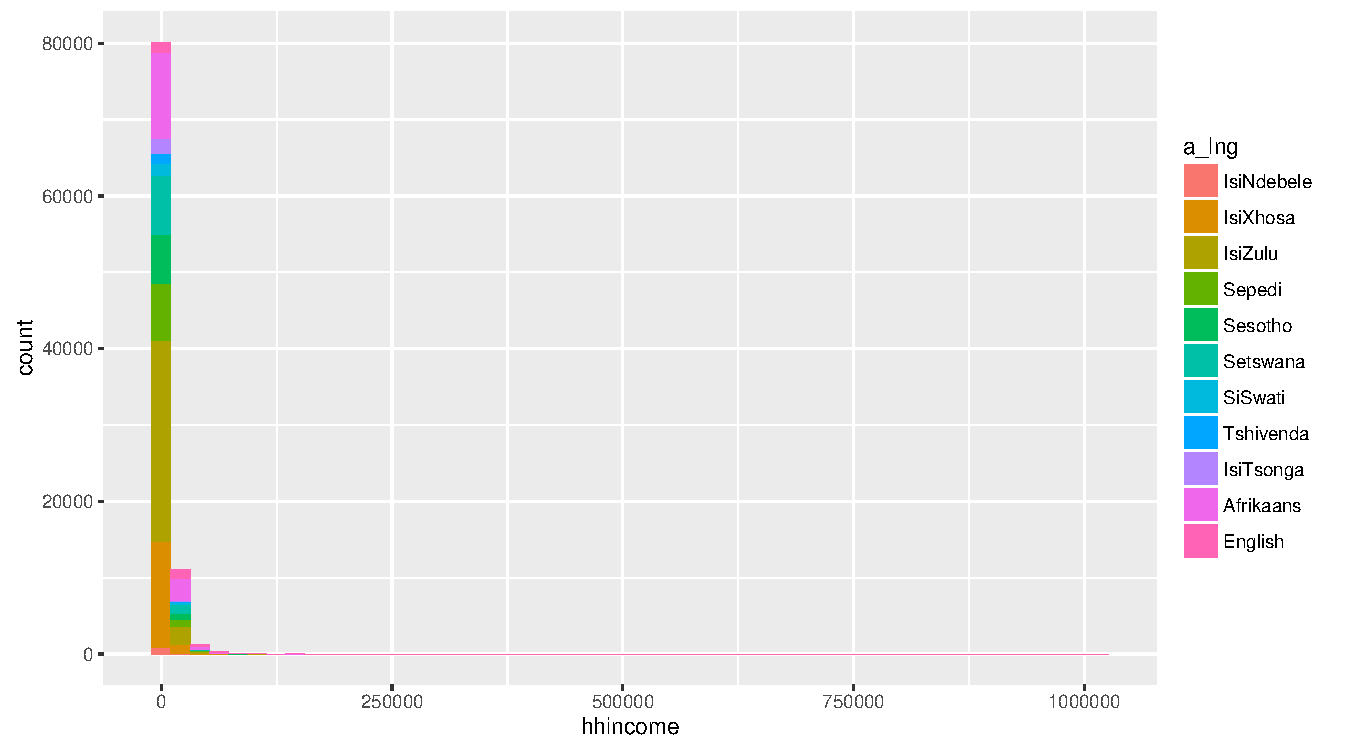
\includegraphics[width=\maxwidth]{../misc/latex-hhincome-1} 

\end{knitrout}
\end{figure}

\begin{figure}[H]
\caption{Years of Education}

\label{fig:bestedu}

\begin{knitrout}
\definecolor{shadecolor}{rgb}{0.969, 0.969, 0.969}\color{fgcolor}\begin{kframe}
\begin{alltt}
\hlkwd{ggplot}\hlstd{(adulthh,} \hlkwd{aes}\hlstd{(}\hlkwc{x}\hlstd{=best_edu,} \hlkwc{fill}\hlstd{=a_lng ))} \hlopt{+}
    \hlkwd{geom_bar}\hlstd{(}\hlkwc{position} \hlstd{=} \hlstr{'fill'}\hlstd{)}
\end{alltt}
\end{kframe}
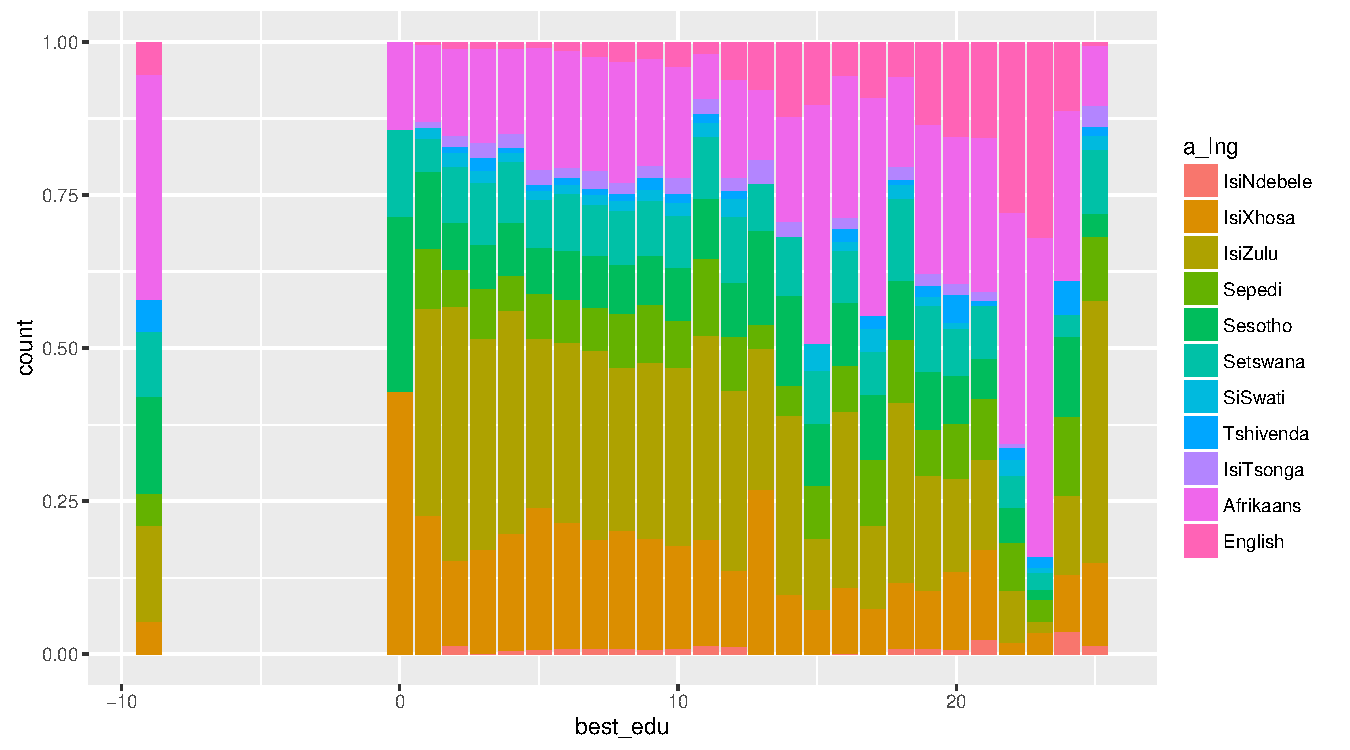
\includegraphics[width=\maxwidth]{../misc/latex-best_edu-1} 

\end{knitrout}
\end{figure}

The \ref{fig:rden} describes the skill of individuals in reading
the English language, where 1 the best and 4 is the worst, grey values
are \code{NA}.

\begin{figure}[H]
\caption{English Language Reading Skills}
\label{fig:rden}

\begin{knitrout}
\definecolor{shadecolor}{rgb}{0.969, 0.969, 0.969}\color{fgcolor}\begin{kframe}
\begin{alltt}
\hlkwd{ggplot}\hlstd{(adulthh,} \hlkwd{aes}\hlstd{(}\hlkwc{x} \hlstd{= a_lng,} \hlkwc{fill} \hlstd{=} \hlkwd{factor}\hlstd{(a_edlitrden)) )} \hlopt{+}
        \hlkwd{geom_bar}\hlstd{(}\hlkwc{position} \hlstd{=} \hlstr{'fill'}\hlstd{)}
\end{alltt}
\end{kframe}
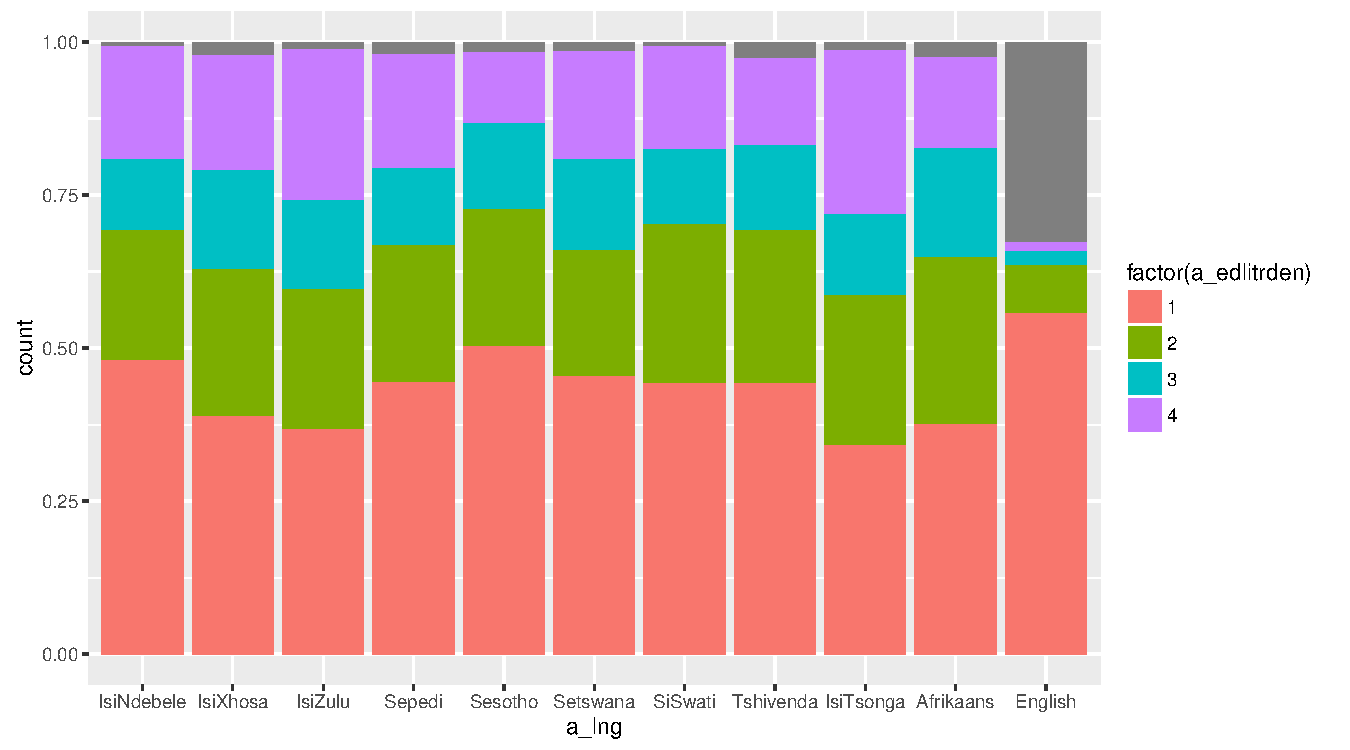
\includegraphics[width=\maxwidth]{../misc/latex-read_english-1} 

\end{knitrout}
\end{figure}

The \ref{fig:rdhm} does the same but with regards to the native language.

\begin{figure}[H]
\caption{Native Language Reading Skills}
\label{fig:rdhm}

\begin{knitrout}
\definecolor{shadecolor}{rgb}{0.969, 0.969, 0.969}\color{fgcolor}\begin{kframe}
\begin{alltt}
\hlkwd{ggplot}\hlstd{(adulthh,} \hlkwd{aes}\hlstd{(}\hlkwc{x} \hlstd{= a_lng,} \hlkwc{fill} \hlstd{=} \hlkwd{factor}\hlstd{(a_edlitrdhm)) )} \hlopt{+}
        \hlkwd{geom_bar}\hlstd{(}\hlkwc{position} \hlstd{=} \hlstr{'fill'}\hlstd{)}
\end{alltt}
\end{kframe}
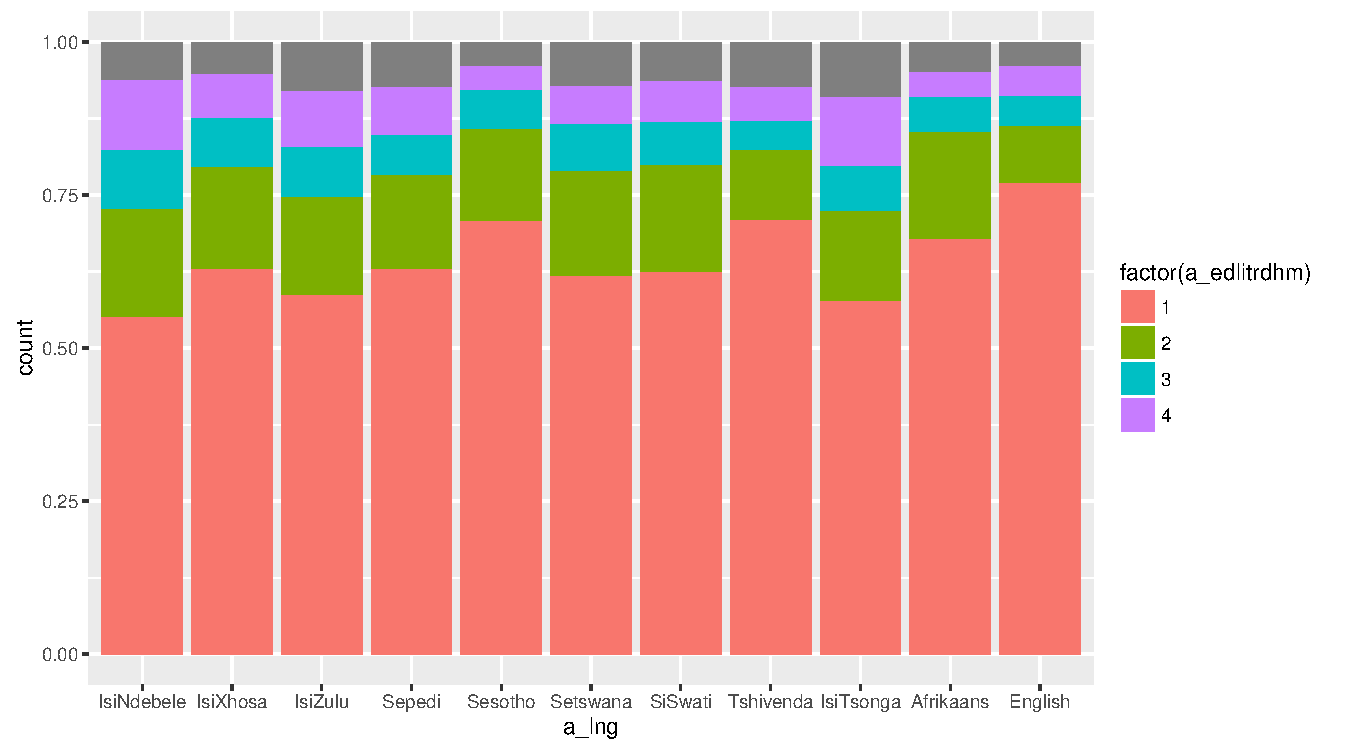
\includegraphics[width=\maxwidth]{../misc/latex-read_native-1} 

\end{knitrout}
\end{figure}


\section{Original Estimates}

\begin{table}[H]
\caption{Computer Ownership}
\label{tab:owncom}

\begin{knitrout}
\definecolor{shadecolor}{rgb}{0.969, 0.969, 0.969}\color{fgcolor}\begin{kframe}
\begin{alltt}
\hlkwd{lm}\hlstd{(a_owncom} \hlopt{~} \hlstd{event}\hlopt{*}\hlstd{setswana}       \hlopt{+}
              \hlkwd{factor}\hlstd{(a_edlitrden)}  \hlopt{+}
              \hlkwd{factor}\hlstd{(a_edlitwrten)} \hlopt{+}
              \hlkwd{factor}\hlstd{(a_edlitrdhm)}  \hlopt{+}
              \hlkwd{factor}\hlstd{(a_edlitwrthm)} \hlopt{+}
              \hlstd{a_woman}              \hlopt{+}
              \hlstd{hhincome}             \hlopt{+}
              \hlstd{best_edu              )}
\end{alltt}
\begin{verbatim}
## 
## Call:
## lm(formula = a_owncom ~ event * setswana + factor(a_edlitrden) + 
##     factor(a_edlitwrten) + factor(a_edlitrdhm) + factor(a_edlitwrthm) + 
##     a_woman + hhincome + best_edu)
## 
## Coefficients:
##            (Intercept)               eventTRUE            setswanaTRUE  
##              9.595e-03              -6.159e-03              -1.551e-02  
##   factor(a_edlitrden)2    factor(a_edlitrden)3    factor(a_edlitrden)4  
##             -3.234e-02              -3.416e-02              -3.928e-02  
##  factor(a_edlitwrten)2   factor(a_edlitwrten)3   factor(a_edlitwrten)4  
##             -1.857e-02              -2.028e-02              -2.048e-02  
##   factor(a_edlitrdhm)2    factor(a_edlitrdhm)3    factor(a_edlitrdhm)4  
##              3.507e-03               2.144e-04              -2.934e-02  
##  factor(a_edlitwrthm)2   factor(a_edlitwrthm)3   factor(a_edlitwrthm)4  
##             -1.133e-03              -5.473e-03              -3.988e-02  
##            a_womanTRUE                hhincome                best_edu  
##             -2.697e-02               5.444e-06               6.174e-03  
## eventTRUE:setswanaTRUE  
##              2.354e-02
\end{verbatim}
\end{kframe}
\end{knitrout}
\end{table}

\begin{table}[H]
\caption{Living in Household that Spent on Internet (last 30 days)}
\label{tab:nfnet}

\begin{knitrout}
\definecolor{shadecolor}{rgb}{0.969, 0.969, 0.969}\color{fgcolor}\begin{kframe}
\begin{alltt}
\hlkwd{lm}\hlstd{(h_nfnet} \hlopt{~}  \hlstd{event}\hlopt{*}\hlstd{setswana_logical} \hlopt{+}
              \hlkwd{factor}\hlstd{(a_edlitrden)}    \hlopt{+}
              \hlkwd{factor}\hlstd{(a_edlitwrten)}   \hlopt{+}
              \hlkwd{factor}\hlstd{(a_edlitrdhm)}    \hlopt{+}
              \hlkwd{factor}\hlstd{(a_edlitwrthm)}   \hlopt{+}
              \hlstd{a_woman}                \hlopt{+}
              \hlstd{hhincome}               \hlopt{+}
              \hlstd{best_edu                )}
\end{alltt}
\begin{verbatim}
## 
## Call:
## lm(formula = h_nfnet ~ event * setswana_logical + factor(a_edlitrden) + 
##     factor(a_edlitwrten) + factor(a_edlitrdhm) + factor(a_edlitwrthm) + 
##     a_woman + hhincome + best_edu)
## 
## Coefficients:
##                    (Intercept)                       eventTRUE  
##                     -1.648e-03                      -1.182e-02  
##           setswana_logicalTRUE            factor(a_edlitrden)2  
##                     -1.343e-02                       2.765e-03  
##           factor(a_edlitrden)3            factor(a_edlitrden)4  
##                     -5.328e-05                      -2.713e-03  
##          factor(a_edlitwrten)2           factor(a_edlitwrten)3  
##                     -9.184e-03                      -8.723e-03  
##          factor(a_edlitwrten)4            factor(a_edlitrdhm)2  
##                     -5.862e-03                      -7.155e-04  
##           factor(a_edlitrdhm)3            factor(a_edlitrdhm)4  
##                     -8.317e-04                      -5.699e-03  
##          factor(a_edlitwrthm)2           factor(a_edlitwrthm)3  
##                     -1.117e-03                      -1.265e-03  
##          factor(a_edlitwrthm)4                     a_womanTRUE  
##                     -9.399e-03                      -6.753e-04  
##                       hhincome                        best_edu  
##                      2.743e-06                       1.295e-03  
## eventTRUE:setswana_logicalTRUE  
##                      1.201e-02
\end{verbatim}
\end{kframe}
\end{knitrout}
\end{table}


\section{Interaction with woman variable}

\begin{table}[H]
\caption{Women Owning a Computer}

\begin{knitrout}
\definecolor{shadecolor}{rgb}{0.969, 0.969, 0.969}\color{fgcolor}\begin{kframe}
\begin{alltt}
\hlkwd{lm}\hlstd{(a_owncom} \hlopt{~} \hlstd{a_woman}\hlopt{*}\hlstd{event}\hlopt{*}\hlstd{setswana} \hlopt{+}
              \hlkwd{factor}\hlstd{(a_edlitrden)}    \hlopt{+}
              \hlkwd{factor}\hlstd{(a_edlitwrten)}   \hlopt{+}
              \hlkwd{factor}\hlstd{(a_edlitrdhm)}    \hlopt{+}
              \hlkwd{factor}\hlstd{(a_edlitwrthm)}   \hlopt{+}
              \hlstd{hhincome}               \hlopt{+}
              \hlstd{best_edu                )}
\end{alltt}
\begin{verbatim}
## 
## Call:
## lm(formula = a_owncom ~ a_woman * event * setswana + factor(a_edlitrden) + 
##     factor(a_edlitwrten) + factor(a_edlitrdhm) + factor(a_edlitwrthm) + 
##     hhincome + best_edu)
## 
## Coefficients:
##                        (Intercept)                         a_womanTRUE  
##                          6.319e-03                          -2.144e-02  
##                          eventTRUE                        setswanaTRUE  
##                         -1.907e-03                          -2.058e-02  
##               factor(a_edlitrden)2                factor(a_edlitrden)3  
##                         -3.239e-02                          -3.425e-02  
##               factor(a_edlitrden)4               factor(a_edlitwrten)2  
##                         -3.946e-02                          -1.852e-02  
##              factor(a_edlitwrten)3               factor(a_edlitwrten)4  
##                         -2.026e-02                          -2.036e-02  
##               factor(a_edlitrdhm)2                factor(a_edlitrdhm)3  
##                          3.470e-03                           1.410e-04  
##               factor(a_edlitrdhm)4               factor(a_edlitwrthm)2  
##                         -2.944e-02                          -1.060e-03  
##              factor(a_edlitwrthm)3               factor(a_edlitwrthm)4  
##                         -5.362e-03                          -3.969e-02  
##                           hhincome                            best_edu  
##                          5.443e-06                           6.176e-03  
##              a_womanTRUE:eventTRUE            a_womanTRUE:setswanaTRUE  
##                         -7.199e-03                           9.321e-03  
##             eventTRUE:setswanaTRUE  a_womanTRUE:eventTRUE:setswanaTRUE  
##                          3.806e-02                          -2.564e-02
\end{verbatim}
\end{kframe}
\end{knitrout}
\end{table}

\newpage{}

\section{Software}

The estimation is primarily performed using R \citep*{R}, specifically
using \code{lm()} and \code{glm()} functions included in the \code{stats}
package \citep{venables2013Splus}. Additionally, I make the of the
\code{plm()} and \code{pglm()} functions which are available in
packages by the same names \citep{croissant2008plm,croissant2013pglm}.
Standard error corrections are computed using the \code{lmtest} and
\code{sandwich} packages \citet{zeileis2002lmtest,zeileis2004sandwichI,zeileis2006sandwichII}.

In order to make the result as easily reproducible as possible, this
research and writing in the article has been done exclusively using
open-source software such as R \citep*{R}. This document is written
and \LyX{} \citep{lyx} in the \LaTeX\citep{lamport1985latex} language
and compiled using the LuaTeX implementation\citep{luatex}. The integration
of R code and output in the document is performed using a process
call literate programming \citet{knuth1984literate} using the knitr
implementation \citet{xie2015knitr} of the Sweave framework \citep{leisch2002sweave}.

All changes are logged using the version control system Git \citep{git}
and publicly available on GitHub at \href{https://github.com/bquast/Making-Next-Billion-Demand-Access/}{https://github.com/bquast/Making-Next-Billion-Demand-Access/}\footnote{The repository can by cloned to a local computer by entering in following
command in a terminal (with Git installed):\\
\code{git clone https://github.com/bquast/Making-Next-Billion-Demand-Access.git}}
\end{document}
